\section{Experiment}
% �����앶�����ق����ǂ�
We confirmed our reward distribution works as expected with a multi-agent setting in ViZDoom \citep{kempka2016vizdoom}, 
an emulator of Doom which have a map editor.
In the setting, additional agents complement the main player.
A player in ViZDoom environment should seek the enemy in the map, and then defeat the enemy.

\subsection{Setup}
We used a scenario based on Defend the Center (DtC), provided by ViZDoom platform.
In DtC, players are placed in the center of a field of circle. They attack enemies that come from the wall.
The game has two players: a main player and a cameraman.
Alhough the main player can attack the enemy with bullets, 
the cameraman has no way to attack, and only scouts for the enemy.
The action space for the main player is the combination of \{ attack, turn left, turn right \}. Therefore, the total number of actions is $2^3 = 8$.
The cameraman has two possible actions: \{ turn left, turn right \}.
Although the players can only change direction, they cannot move on the field.
The enemy will die if have the attack (bullet) from the main player once, then player receives +1.
As a default on an episode, the ammunition amount is 26.
The main player will die if under attack from the enemy to the extent that health becomes 0, then the player receives -1.
The cameraman will not die if attacked by the enemy.
The episode will terminate when the maim player dies, or after 525 steps have elapsed.

\subsection{Model}
We compared three models: the proposed method and two comparison targets.

{\em Baseline}: DQN without communication. The main player learns standard DQN with the perspective that the player is viewing.
Because the cameraman does not learn, the player continues to move randomly.

{\em Comm}: DQN with communication. The main player learns DQN with two perspectives: the player's own and the cameraman's.
The communication vector is learned with a feed-forward neural network. The method is inspired by Commnet.

{\em NaaA}: The proposed method. The main player learns DQN with two perspectives: the player's own and the cameraman's.
The transmission of reward and communication are performed using the proposed method.

\begin{figure*}[t]
\centering
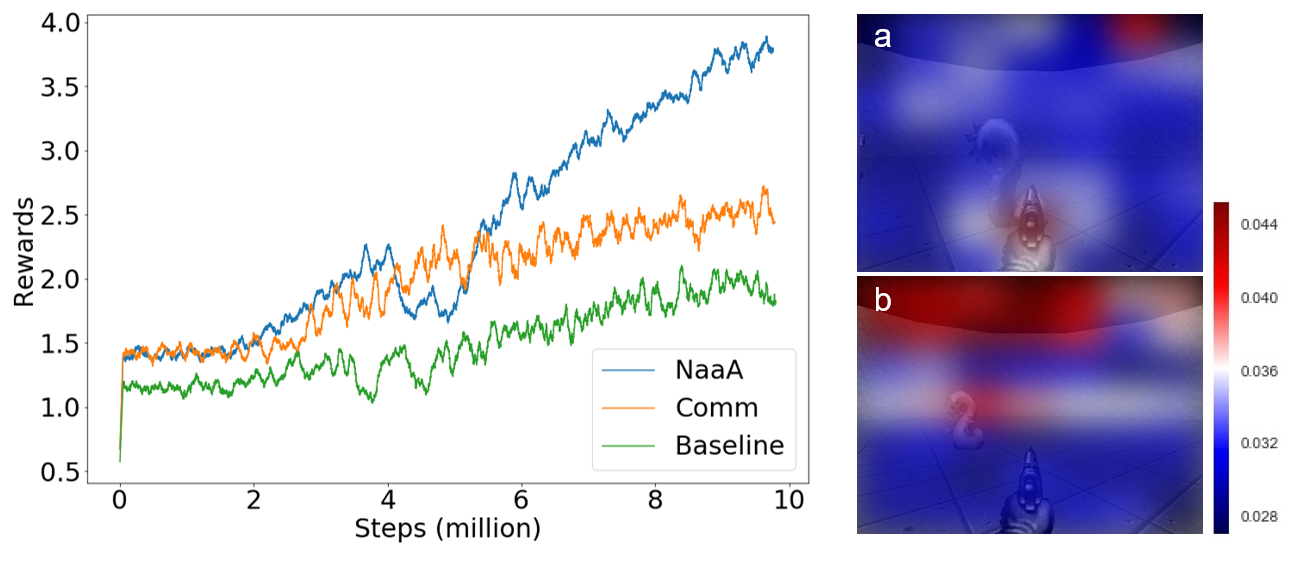
\includegraphics[width=\linewidth]{img/lc_vis.eps}
\caption{
	\textbf{Left:}
		Learning curve for the multi-agent task of VizDoom. 
		Our method based on NaaA outperforms the other two methods: baseline and Comm DQN.
	\textbf{Right:} 
		Visualizing reward from the main player to the cameramann shows us what is important information for the main player:
		(a) The cameraman sees the pistol.
		(b) The cameraman sees the point which enemy appear and come closer.
}
\label{fig:lc_vis}
\end{figure*}

\begin{figure*}[t]
\centering
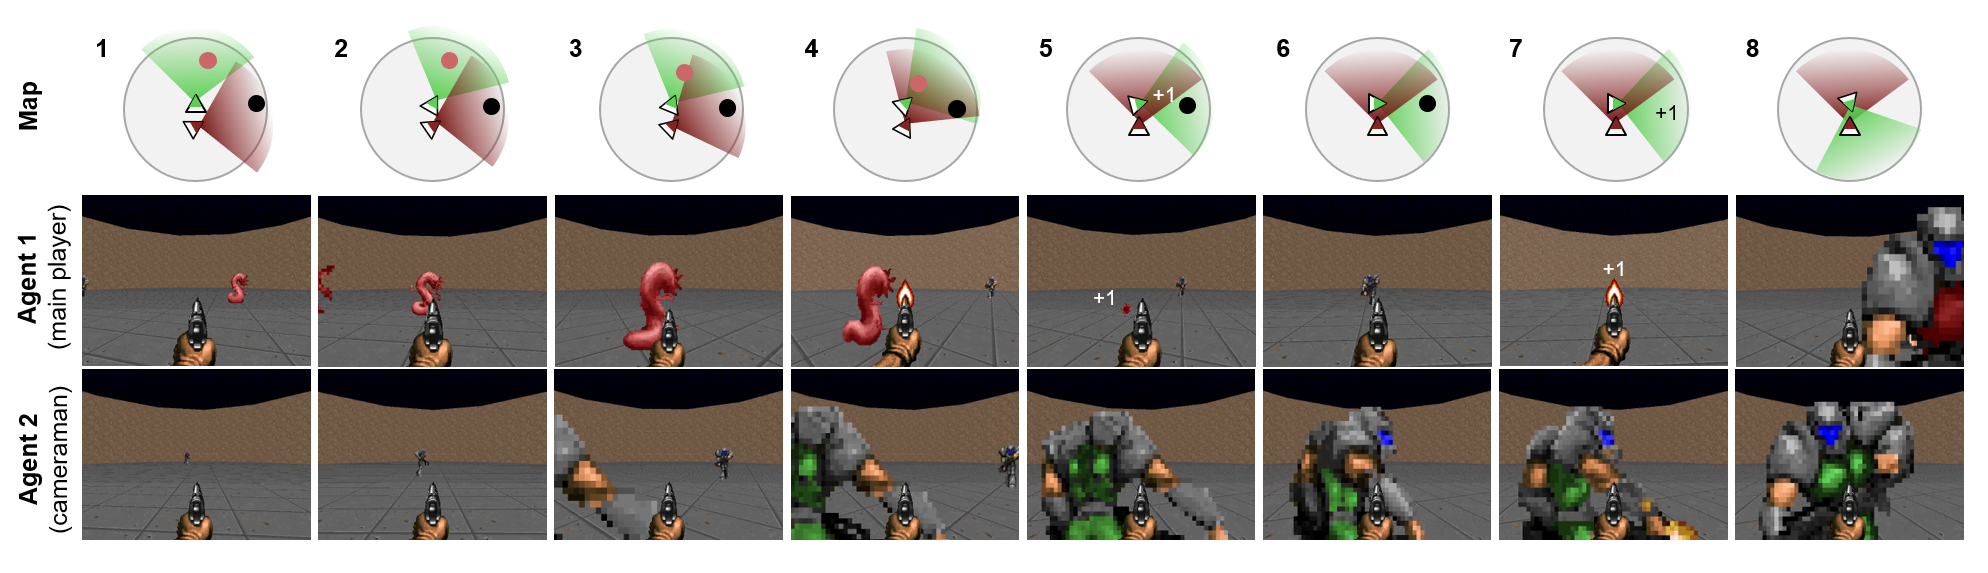
\includegraphics[width=\linewidth]{img/circleworld.eps}
\caption{
NaaA leads the agents to obtain cooperative relationship.
First, the two agents are facing in different directions,
and the cameraman sells its information to the main player (\textbf{1}).
The main player who bought the information starts to turn right to find the enemy.
The cameraman who sold the information starts to turn left to seek new information by finding the blind area of the main player (\textbf{2} and \textbf{3}).
With turning, the main player attacks the first enemy which he already saw (\textbf{4} and \textbf{5}).
After the main player finds out the enemy, he attacks the enemy, and obtain the reward  (\textbf{6} and \textbf{7}).
Until the next enemy appears, the agents watch their dead area each other (\textbf{8}).
}
\label{fig:circleworld}
\end{figure*}

\subsection{Results}
Training is performed in 10 million steps.
Figure \ref{fig:lc_vis} Left presents that our model NaaA outperforms two methods.
Improvement is achieved by Adaptive DropConnect.
We confirmed that the cameraman sees the enemy through an episode.
This can be interpreted as the cameraman reporting the enemy position.
In addition to seeing the enemy, the cameraman sees the area behind of main player several times.
This action enables the cameraman to observe attacks from the enemy while seizing a better relative position.

For further interpretation of the result, 
we present visualization of the revenue that the agent earned in Figure \ref{fig:lc_vis} Right as a heatmap.
The background picture is a screen in Doom taken at the moment when the filter in CNN is mostly activated.
%The center corresponds to a position with the enemy appearing far away.
%The top corresponds to a position with the enemy coming closer.
%(b) shows that the agent sees the pistol.
Figure \ref{fig:circleworld} shows an example of learnt sequence of actions by our method.


%To confirm that NaaA works widely with machine learning tasks,
%we confirm our method of supervised learning tasks as well as reinforcement learning tasks.
%As supervised learning tasks, we use typical machine learning tasks such as image classification
%using MNIST, CIFAR-10, and SVHN.

%As reinforcement tasks, we confirm single- and multi-agent environment.
%The single-agent environment is from OpenAI gym.
%We confirm the result using a simple reinforcement task: CartPole.
%In multi-agent, we use ViZDoom, a 3D environment for reinforcement learning.

%The additional feature of NaaA is credit assignment for reward distribution, 
%meaning that if the neural network is divided into multiple agents, it works by playing the auction game.
